\RequirePackage[hyphens]{url}
\documentclass[a4paper,12pt]{article}
\usepackage[OT4]{polski}
\usepackage[utf8]{inputenc}  
\usepackage[top=2cm, bottom=2cm, left=2cm, right=2cm]{geometry}
\usepackage{setspace}

\usepackage{tabu}
\usepackage{longtable}
\usepackage[table]{xcolor}

\usepackage{hyperref}

\usepackage{graphicx} 
\usepackage{minted}
\usemintedstyle{xcode}
\usepackage{algorithmic}
\usepackage{amsmath}

\usepackage[hyphens]{url}
\usepackage{hyperref}
\expandafter\def\expandafter\UrlBreaks\expandafter{\UrlBreaks%  save the current one
	\do\a\do\b\do\c\do\d\do\e\do\f\do\g\do\h\do\i\do\j%
	\do\k\do\l\do\m\do\n\do\o\do\p\do\q\do\r\do\s\do\t%
	\do\u\do\v\do\w\do\x\do\y\do\z\do\A\do\B\do\C\do\D%
	\do\E\do\F\do\G\do\H\do\I\do\J\do\K\do\L\do\M\do\N%
	\do\O\do\P\do\Q\do\R\do\S\do\T\do\U\do\V\do\W\do\X%
	\do\Y\do\Z}

\definecolor{tableHeader}{RGB}{211, 47, 47}
\definecolor{tableLineOne}{RGB}{245, 245, 245}
\definecolor{tableLineTwo}{RGB}{224, 224, 224}

\newcommand{\tableHeaderStyle}{
	\rowfont{\leavevmode\color{white}\bfseries}
	\rowcolor{tableHeader}
}


\makeatletter
\newcommand{\linia}{\rule{\linewidth}{0.4mm}}

\renewcommand{\maketitle}{\begin{titlepage}		
		
		\begin{flushleft}\large
			\@author \hspace{0.5cm} 225961 \hspace{\stretch{1}}
			\textbf{Termin: } Wtorek TP 8:00\\
		\end{flushleft}
		
		\vspace{1.5cm}
		
		\begin{center}
			\begin{figure}[h]
				\centering
\includegraphics[width=4cm]{Materialy/PWR}
				\label{fig:PWR}
			\end{figure}
		\end{center}	
		\centering\Huge Politechnika Wrocławska\\
		\centering\LARGE Wydział Elektroniki\\
		
		\vspace{2.5cm}
		
		\noindent\linia
		\begin{center}	
			\LARGE \textsc{\@title}\\
			\vspace{0.3cm}
			\Large Sprawozdania z laboratoriów
		\end{center}
		\linia
		
		\begin{center}
			\vspace{3cm}	
			\large Prowadząca:\\
			\Large Mgr inż. Aleksandra Postawka
		\end{center}
		
		\vspace*{\stretch{6}}
		
		\begin{center}		
			\large \@date
		\end{center}
		
	\end{titlepage}%
	
}

\makeatother

\begin{document}
	
	\taburowcolors[2] 2{tableLineOne .. tableLineTwo}
	\tabulinesep = ^4mm_4mm
	\everyrow{\tabucline[.4mm  white]{}}
	
	\title{Organizacja i Architektura Komputerów}
	\author{Kamil Dobrysiewicz}
	\date{17.06.2019}
	\maketitle
	
\newpage
	
	
\tableofcontents
\newpage
	
\section{(0) Wprowadzenie do zajęć}
\subsection{Treść ćwiczenia}
\textbf{Zakres i program ćwiczenia:}
\begin{itemize}
	\item Podstawy poruszania się po systemie Linux - komendy \textbf{man, cd, ls, rm, cat} itp.
	\item Podstawy składni programów dla GNU Assembler.
	\item Kompilacja  i konsolidacja programów za pomocą poleceń \textbf{as, ld, gcc}.
	\item Wykorzystanie funkcji standardowych - \textbf{syscall}.
	\item Zdalne logowanie do systemów \textbf{unix}opodobnych za pomocą SSH, Putty, WinSCP.
	\item Pierwszy program "Hello World!".
	\item Modyfikacje programu.
	\item Podstawy obsługi debuggera \textbf{gdb}.
\end{itemize}
\textbf{Zrealizowane zadania:}
\begin{itemize}
	\item Zapoznanie się z działaniem podstawowych komend konsoli systemu Linux Ubuntu.
	\item Zapoznanie się ze składnią programu w języku GNU Assembler.
	\item Zapoznanie się z metodami zdalnego logowania do systemu Linux za pomocą SSH, Putty oraz WinSCP.
	\item Przygotowanie pliku sterującego \textbf{makefile} dla komendy \textbf{make} i gotowego programu "Hello World!".
	\item Przygotowanie programu wczytującego ciąg znaków z klawiatury do bufora, zamieniającego duże litery tego ciągu na małe i odwrotnie oraz wypisującego na ekran zmodyfikowany ciąg wejściowy.
	\item Zapoznanie się z obsługą debuggera \textbf{GDB}. 	
\end{itemize}
\subsection{Przebieg ćwiczenia}
\subsubsection{Utworzenie przestrzeni roboczej}
Przed rozpoczęciem tworzenia programów w języku GNU Assembler konieczne było przygotowanie miejsca do przechowywania programów. W tym celu wykorzystano komendę \textbf{mkdir} do stworzenia folderu o nazwie OiAK. Następnie za pomocą komendy \textbf{cd} ustanowiono nowy folder bieżącą lokalizacją. W tym folderze przechowywane będą podfoldery zawierające programy napisane podczas poszczególnych laboratoriów, zaś cały folder zostanie zapisany w repozytorium GitHub.
\subsubsection{Podstawowe komendy konsoli systemu Linux}
Poza opisanymi w poprzedniej sekcji komendami \textbf{mkdir} oraz \textbf{cd} przetestowano szereg innych komend konsoli systemu Linux Ubuntu:
\begin{itemize}
	\item \textbf{touch} - utworzenie pliku w katalogu bieżącym, np. touch hello.s.
	\item \textbf{cat} - wypisanie na ekran zawartości wybranego pliku, np. cat hello.s wypisze na ekran zawartość pliku hello.s.
	\item \textbf{ls} - wyświetlenie listy plików katalogu bieżącego.
	\item \textbf{rm} - usunięcie pliku lub folderu (dla folderów z zawartością należy użyć dodatkowo opcji \textbf{-rf}).
	\item \textbf{cp} - kopiowanie pliku, np. cp Lab0/hello.s Lab1/hello.s skopiuje plik z katalogu Lab0 do katalogu Lab1.
	\item \textbf{man} - wyświetlenie instrukcji obsługi, np. man ls pokaże instrukcję obsługi komendy ls.
	\item \textbf{code} - uruchomienie edytora Visual Studio Code, z którego korzystano podczas laboratorium.
\end{itemize}
\subsubsection{Składnia programu GNU Assembler}
W programie napisanym w języku assembler można wyróżnić następujące sekcje kodu:
\begin{itemize}
	\item .data - zawiera ona stałe wykorzystywane w programie.
	\item .bss - zawiera deklaracje buforów danych, nieznanych w momencie uruchomienia programu.
	\item .text - zawiera kod programu.
\end{itemize}
Programy napisane w języku GNU Assembler wymagają podania tzw. punktu wejścia do programu. Zadanie to realizuje się poprzez napisanie w sekcji \textbf{.text} dyrektywy \textbf{.globl} ze słowem \_start (dla as i ld) lub main (dla gcc). W opisywanych programach kompilacja odbywa się za pomocą gcc, dlatego też punkt startowy wskazuje \textbf{.globl main}.
\newpage
\subsubsection{Metody zdalnego logowania do systemu Linux}
System Linux pozwala na zdalne zalogowanie za pomocą następujących metod:
\begin{enumerate}
	\item SSH - umożliwia zdalne zalogowanie do systemu Linux z poziomu konsoli uruchomionej na innym urządzeniu z systemem Linux.
	\begin{center}
		\begin{figure}[h]
			\centering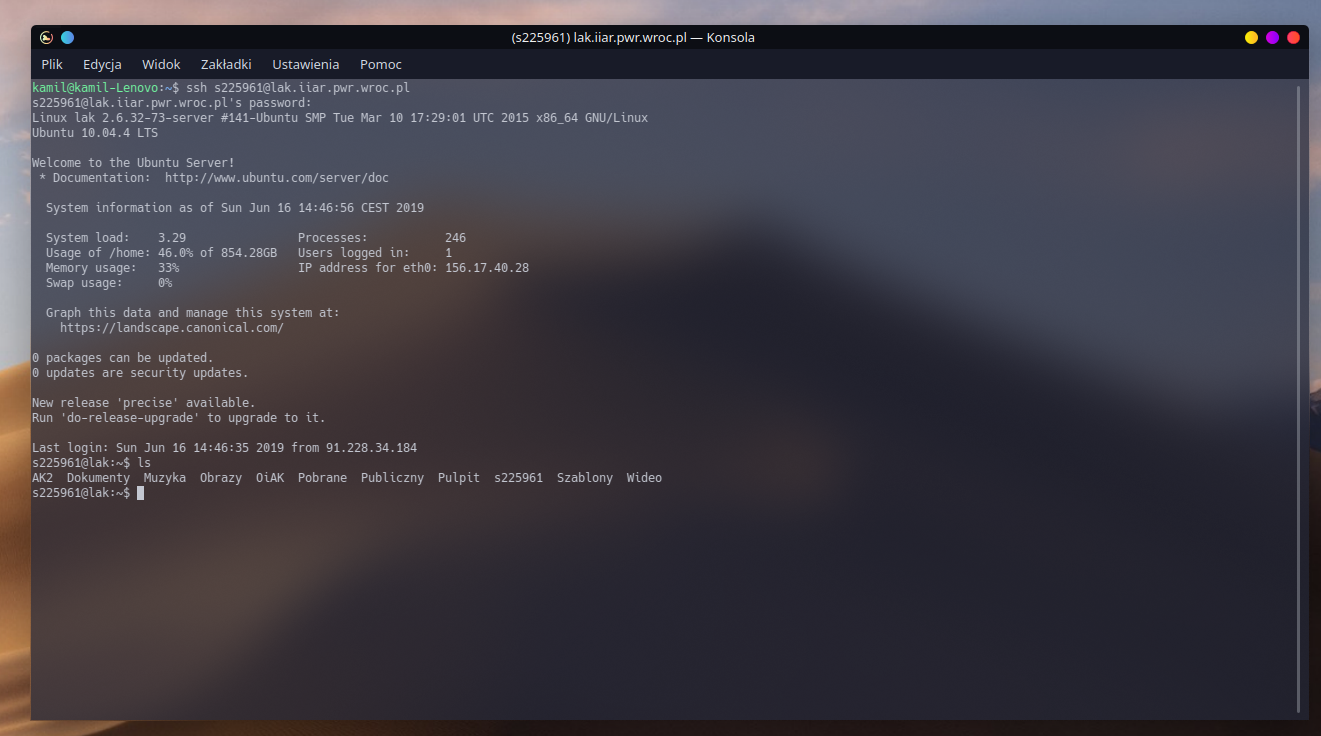
\includegraphics[width=17cm]{Materialy/Lab0/ssh}
			\caption{Zdalne logowanie do systemu za pomocą SSH}
			\label{ssh}
		\end{figure}
	\end{center}
	\item Putty - pozwala na zalogowanie się do konsoli systemu Linux z poziomu systemu Windows.
	\item WinSCP - aplikacja umożliwiająca łatwą wymianę plików pomiędzy systemem Windows, a zdalnie zalogowanym systemem Linux (pośrednio za pomocą Putty).
\end{enumerate}
Podczas realizacji zadań laboratoryjnych nie korzystano z możliwości zdalnego logowania. Korzystano z prywatnego laptopa z zainstalowanym systemem Linux Ubuntu 19.04 z nakładką graficzną KDE Plasma (Kubuntu 19.04).
\subsubsection{Plik sterujący makefile oraz wywołanie programu}
W celu uruchomienia gotowej aplikacji "Hello World!" konieczne było przygotowanie pliku sterującego dla programu make, tzw. \textbf{makefile}. Jego struktura przedstawiona została na poniższym listingu:
\begin{minted}{bash}
hello:	hello.o
	ld -o hello hello.o

hello.o:	hello.s
	as -o hello.o hello.s
\end{minted}
W pliku makefile wywołano kompilator \textbf{as} oraz konsolidator \textbf{ld}. Bardzo ważne jest odpowiednie umiejscowienie tabulatorów w pliku makefile. Bez tego wywołanie programu \textbf{make} może się nie powieść.  Wywołanie programu \textbf{make} w katalogu, w którym znajdują się pliki hello.s oraz makefile spowoduje stworzenie pliku wykonywalnego \textbf{hello}, który uruchomić można za pomogą komendy:\\\\ \textbf{./hello}.\\\\ Oznacza to uruchomienie programu \textbf{hello}, znajdującego się w katalogu bieżącym.\\
Korzystanie z makefile może być uznawane za wygodne. Istnieje jednak inny sposób kompilacji programu. Zamiast \textbf{as} i \textbf{ld} zastosować można kompilator \textbf{gcc}, który pozwala na znaczne uproszczenie procesu generowania pliku wykonywalnego z programem. Dla pliku hello.s wystarczy użyć komendy:\\\\
\textbf{gcc -no-pie -g -o hello hello.s}.\\\\
Opcja -g jest opcjonalna, umożliwia dodanie informacji dla debuggera. Opcja -no-pie jest zaś niezbędna do kompilacji programu na nowszych systemach. W systemie zainstalowanych w laboratorium nie jest konieczna.\\
Wszystkie programy stworzone w ramach realizacji laboratorium kompilowane są za pomocą gcc, sposób ten został uznany przez autora aplikacji za wygodniejszy.
\subsubsection{Program modyfikujący ciąg znaków}
W ramach zadania domowego przygotowany został program wykorzystujący funkcje standardowe systemu Linux (SYSREAD, SYSWRITE oraz SYSEXIT). Wczytuje on ciąg znaków z klawiatury, zamienia wszystkie małe litery na duże i odwrotnie, a następnie wypisuje wynik na wyjście standardowe. Kod programu przedstawiono na listingu:
\begin{minted}{gas}
	.data 
	STDIN = 0
	STDOUT = 1
	SYSREAD = 0
	SYSWRITE = 1
	SYSEXIT = 60
	EXIT_CODE = 0
	TEXT_TO_CHANGE_LENGTH = 512
	TEXT_TO_PRINT_LENGTH = 512
	
	TEXT: .ascii "Insert some text:\n"
	TEXT_LENGTH = .-TEXT
	WRITE_TEXT: .ascii "Your text after change is: \n"
	WRITE_TEXT_LENGTH = .-WRITE_TEXT
	
	.bss
	.comm TEXT_TO_CHANGE, 512 # Bufor wejściowy i jego rozmiar
	.comm TEXT_TO_PRINT, 512 # Bufor wyjściowy i jego rozmiar
	
	
	
	
	.text
	.globl main
	
	main:
	
	... # Wydrukowanie komunikatu dla użytkownika
	
	# Pobranie danych z wejścia standardowego
	movq $SYSREAD, %rax  # Kod funkcji systemowej
	movq $STDIN, %rdi # Kod wejścia standardowego
	movq $TEXT_TO_CHANGE, %rsi # Adres bufora wejściowego
	movq $TEXT_TO_CHANGE, %rdx # Rozmiar bufora wejściowego
	syscall

		
	dec %rax # Liczba wczytanych bajtów - 1 w %rax
	xorq %rdi, %rdi # Wyzerowanie rejestru %rdi - licznika pętli 
	
	loop_start: # Pętla
	# Skopiowanie jednego znaku z bufora wejściowego do rejestru %bl
	movb TEXT_TO_CHANGE(, %rdi, 1), %bl
	cmpb $'a', %bl
	# Kod znaku < 'a' - skok do sprawdzenia, czy znak jest dużą literą.
	jl maybe_big_letter
	cmpb $'z', %bl
	# Kod znaku > 'z' - inny znak - skok do przepisania
	jg other_sign
	
	# Mała litera
	andb $0xDF, %bl # Zamiana na dużą literę
	movb %bl, TEXT_TO_PRINT(, %rdi, 1) # Zapis do bufora wyjściowego
	jmp end_loop
	
	
	maybe_big_letter:
	cmpb $'A', %bl
	# Kod litery < 'A' - inny znak - skok do przepisania
	jl other_sign
	cmpb $'Z', %bl
	# Kod litery > 'Z' - inny znak - skok do przepisania
	jg other_sign
	
	# Duża litera
	xorb $0x20, %bl # Zamiana na małą literę
	movb %bl, TEXT_TO_PRINT(, %rdi, 1) # Zapis do bufora wyjściowego
	jmp end_loop
	
	# Inny znak
	other_sign:
	movb %bl, TEXT_TO_PRINT(, %rdi, 1) # Zapis do bufora wyjściowego
	
	# Sprawdzenie warunku końca pętli
	end_loop:
	inc %rdi # Zwiększenie licznika
	cmp %rax, %rdi # Porównanie do liczby wczytanych bajtów - 1
	jl loop_start # Jeśli %rdi < %rax - skok do początku pętli
	
	# Dopisanie znaku końca linii do tekstu wynikowego.
	movb $'\n', TEXT_TO_PRINT(, %rdi, 1)
	
	... # Wydrukowanie komunikatu dla użytkownika
	
	# Wypisanie tekstu z bufora.
	movq $SYSWRITE, %rax
	movq $STDOUT, %rdi
	movq $TEXT_TO_PRINT, %rsi
	movq $TEXT_TO_PRINT_LENGTH, %rdx
	syscall
	
	# Zakończenie działania programu.
	movq $SYSEXIT, %rax 
	movq $EXIT_CODE, %rdi # Kod zwracany przez program
	syscall
	
\end{minted}
W sekcji \textbf{.data} zadeklarowane zostały stałe przechowujące kody funkcji systemowych, wejścia i wyjścia standardowego oraz dodatkowe komunikaty drukowane przez program. Sekcja \textbf{.bss} przechowuje deklaracje dwóch buforów: jeden dla tekstu wprowadzanego przez użytkownika, a drugi dla tekstu przetworzonego przez program.\\
Następnie w kodzie zauważyć można punkt wejścia do programu (main dla gcc). W kolejnym kroku program pobiera z wejścia standardowego ciąg znaków do przetworzenia. Wykorzystana została funkcja systemowa \textbf{SYSREAD}, której kod zapisano w rejestrze \textbf{\%rax}. W rejestrze \textbf{\%rdi} zapisany został kod wejścia standardowego, w \textbf{\%rsi} - adres bufora, do którego ma zostać zapisany odczytany ciąg znaków, a w \textbf{\%rdx} - rozmiar bufora w bajtach. Funkcję systemowe wywoływane są za pomocą przerwania programowego \textbf{syscall}. Po wywołaniu przerwania systemowego w rejestrze \textbf{\%rax} znajduje się ilość bajtów wczytanych przez funkcję.\\
Dalsza część programu ma za zadanie przetworzenie odczytanego tekstu. W pętli pobiera kolejne bajty danych, sprawdza, jaki znak aktualnie przetwarza i dokonuje odpowiedniej konwersji - z małej litery na dużą, z dużej na małą, bądź przepisuje znak bez modyfikacji. Wynik przetworzenia zapisywany jest w buforze wyjściowym \textbf{TEXT\_TO\_PRINT}.\\
Na koniec zawartość bufora wyjściowego wypisywana jest na ekran za pomocą funkcji systemowej \textbf{SYSWRITE}, której wywołanie jest podobne do wcześniej opisanego \textbf{SYSREAD}.\\
Zamknięcie programu dokonywane jest przy pomocy kolejnej funkcji systemowej - \textbf{SYSEXIT}. W rejestrze \textbf{\%rdi} przechowywany jest kod błędu, który po zakończeniu programu można podejrzeć w konsoli za pomogą komendy \textbf{echo \$?}.

\subsubsection{Zapoznanie się z obsługą debuggera}
Debugger to bardzo przydatne narzędzie, które pozwala na bieżąco podglądać zawartość poszczególnych rejestrów podczas działania programu i umożliwia odnalezienie błędów w przypadku ich wystąpienia. Po kompilacji programu z uwzględnieniem informacji dla debuggera (opcja -g dla gcc) możliwe jest uruchomienie aplikacji w gdb za pomocą komendy:\\\\
\textbf{gdb zad1}.\\\\
Po załadowaniu programu należy wybrać miejsca, w których program ma być zatrzymywany (ang. breakpoint). W tym celu należy wpisać komendę \textbf{b 20}, gdzie 20 oznacza numer linii kodu programu, w której program ma być zatrzymany. Możliwe jest dodanie wielu punktów przerwania programu. Po dodaniu breakpointów można wykonać program za pomocą komendy \textbf{run} lub w skrócie \textbf{r}. Program zatrzyma się w pierwszym zdefiniowanym punkcie przerwania, co pokazano na \textit{rysunku 2}.
\begin{center}
	\begin{figure}[h]
		\centering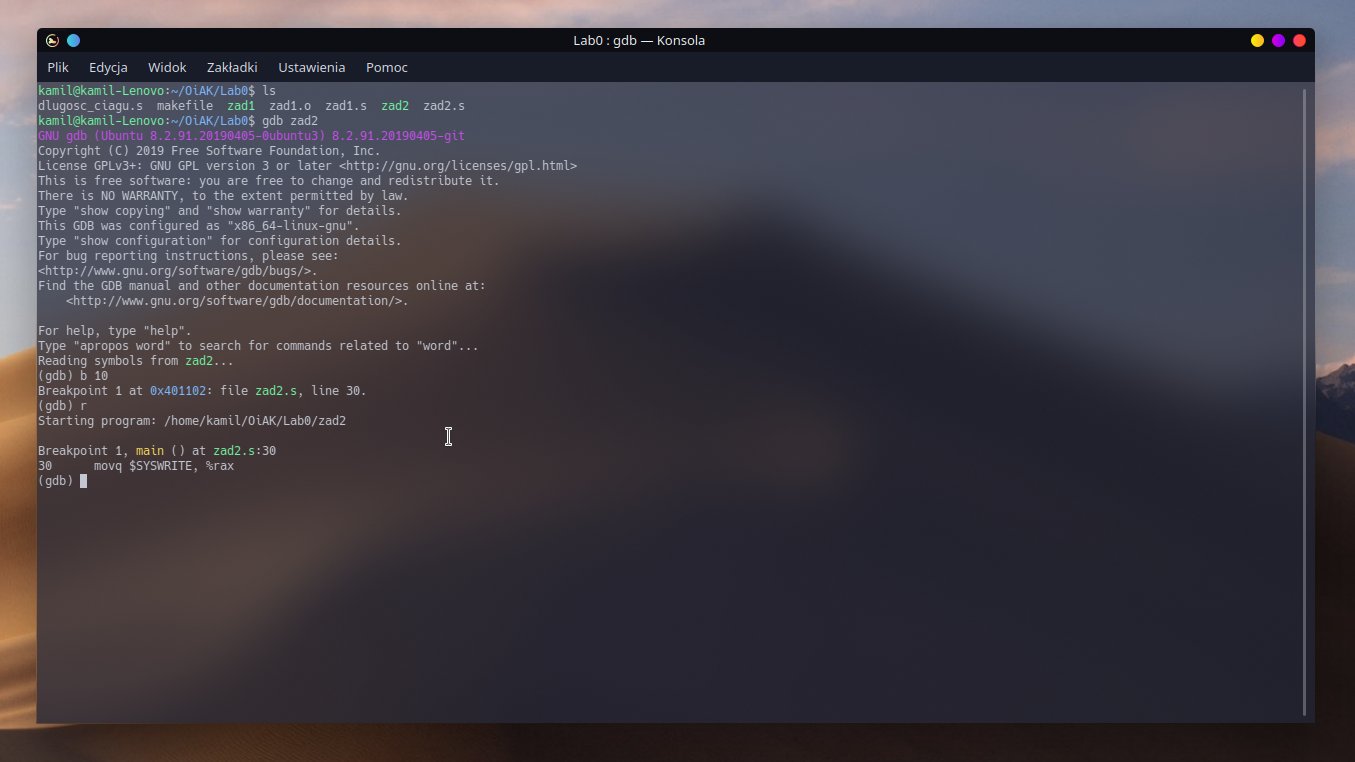
\includegraphics[width=17cm]{Materialy/Lab0/gdb1}
		\caption{Zatrzymanie wykonania programu w gdb}
		\label{gdb1}
	\end{figure}
\end{center}
Wykonanie zatrzymanego programu można wznowić za pomocą komendy \textbf{continue (c)}. Po zatrzymaniu programu w punkcie przerwania możliwy jest podgląd wartości rejestrów, buforów, stosu itp. Służą do tego komendy, takie jak:
\begin{itemize}
	\item info registers (i r) - wyświetla zawartość wszystkich rejestrów programu.
	\item print (p) - wyświetla zawartość pojedynczego rejestru.
	\item x/nsf - wyświetla zawartość bufora (n oznacza liczbę pól, s - rozmiar, f - format).
\end{itemize}
Sesję gdb można zakończyć za pomocą komendy \textbf{quit (q)}.
\subsection{Wnioski}
Laboratorium pozwoliło na zapoznanie się z obsługą wiersza poleceń systemu Linux oraz procesem tworzenia programów w języku GNU Assembler. Wszystkie zadania zostały zrealizowane prawidłowo, przygotowane programy wykonały się poprawnie i nie zwróciły żadnych błędów. 
\section{(1) Pętle, podstawowe operacje logiczne i arytmetyczne}
\subsection{Treść ćwiczenia}
\textbf{Zakres i program ćwiczenia:}
\begin{enumerate}
	\item Program umożliwiający sprawdzenie, czy liczba jest liczbą pierwszą:
	\begin{itemize}
		\item  rejestry 64-bitowe, liczba zapisana w stałej.
		\item  odpowiedni komunikat.
	\end{itemize}
	\item  Program konwertujący liczbę z reprezentacji trójkowej na system dziewiątkowy:
	\begin{itemize}
		\item wczytanie liczby z stdin w reprezentacji trójkowej.
		\item sprawdzenie poprawności wpisanego ciągu.
		\item zamiana na liczbę (podgląd w GDB).
		\item konwersja na system dziewiątkowy w formacie tekstowym i wypisanie na ekran.
	\end{itemize}
\end{enumerate}
\textbf{Zrealizowane zadania:}
Udało się zrealizować wszystkie zadania przewidziane do realizacji w ramach laboratorium.
\subsection{Przebieg ćwiczenia}
\subsubsection{Program umożliwiający sprawdzenie, czy liczba jest liczbą pierwszą}
W celu przygotowania programu sprawdzającego, czy liczba zapisana w pamięci jest liczbą pierwszą w sekcji \textbf{.data} zdefiniowano stałe do wywołania funkcji systemowych \textbf{SYSWRITE} oraz \textbf{SYSEXIT}, liczbę do weryfikacji oraz dwa komunikaty tekstowe, wypisywane na ekran w momencie, gdy liczba jest lub nie jest liczbą pierwszą. Sekcja \textbf{.bss} pozostała pusta.\\
Przygotowany algorytm sprawdza ile testowana liczba ma dzielników. Jeżeli istnieją dokładnie dwa dzielniki testowanej liczby to jest ona liczbą pierwszą. W przeciwnym wypadku nie jest. Realizację algorytmu rozpoczęto od wyzerowania rejestrów \textbf{\%rbx} (Liczba dzielników) oraz \textbf{\%rcx} (aktualnie testowany dzielnik). Następnie przygotowano krótką pętlę, przedstawioną na listingu:
\begin{minted}{gas}
	loop:
	inc %rcx # Inkrementacja dzielnika
	xor %rdx, %rdx # Zerowanie %rdx
	movq $NUMBER, %rax # Przeniesienie liczby z pamięci do rejestru %rax 
	divq %rcx # Dzielenie testowanej liczby przez aktualny dzielnik
	cmpq $0, %rdx # Sprawdzenie, czy reszta wynosi 0
	jne loop # Jeśli reszta jest różna od 0 - skok do początku pętli
	inc %rbx # Inkrementacja wyniku
	# Warunek końca pętli: testowana liczba = aktualnemu dzielnikowi
	cmp $NUMBER, %rcx 
	je end # Jeżeli testowana liczba = aktualny dzielnik - skok poza pętlę
	jmp loop # Skok bezwarunkowy do początku pętli
\end{minted} 
Pętla jest bardzo prosta - za każdym razem pobiera testowaną liczbę z pamięci do rejestru \textbf{\%rcx}, dzieli przez kolejny dzielnik i w zależności od tego, czy wynik dzielenia posiada resztę  - inkrementuje licznik dzielników o jeden lub nie. W każdej iteracji pętli zerowany jest rejestr \textbf{\%rdx}, który przechowuje resztę z dzielenia. Do rejestru \textbf{\%rax} trafia zaś wynik operacji dzielenia. W kodzie realizującym algorytm występują trzy typy skoków warunkowych, poprzedzonych operacją porównania (\textbf{cmp}):
\begin{itemize}
	\item jne - skok, jeżeli porównywane liczby są różne.
	\item je - skok, jeżeli porównywane liczby są równe.
	\item jmp - przypadek szczególny - skok bezwarunkowy.
\end{itemize}
Poza wykorzystanymi w programie istnieją jeszcze inne operacje skoków warunkowych, o których warto wspomnieć:
\begin{itemize}
	\item jl - skok, jeżeli liczba po prawej stronie jest mniejsza od tej po lewej stronie.
	\item jle - skok, jeżeli liczba jest mniejsza lub równa drugiej.
	\item jg - skok, jeżeli liczba jest większa od drugie.
	\item jge - skok, jeżeli liczba jest większa lub równa drugiej.
\end{itemize}
Po zakończeniu pracy pętli, zawartość rejestru przechowującego liczbę dzielników (\textbf{\%rbx}) poddawana jest weryfikacji za pomocą operacji porównania.
\begin{minted}{gas}
	end:
	cmp $2, %rbx # Porównanie, czy wynik w %rbx = 2
	# Jeśli wynik nie jest równy 2 to liczba nie jest pierwsza.
	jne not_prime_number
\end{minted}
Na koniec drukowany jest odpowiedni komunikat za pomocą funkcji systemowej \textbf{SYSWRITE}.
\subsubsection{Program konwertujący liczbę z reprezentacji trójkowej na system dziewiątkowy}
W celu przygotowania programu do konwersji liczb z systemu trójkowego na dziewiątkowy w sekcji \textbf{.data} poza komunikatami dla użytkownika oraz stałymi do wywołania funkcji systemowych, zdefiniowano stałą przechowującą rozmiar buforów, przechowujących liczby w systemach trójkowym oraz dziewiątkowym. W sekcji \textbf{.bss} zdefiniowano dwa bufory, przedstawione na listingu:
\begin{minted}{gas}
	.bss
	# Liczba w systemie trójkowym, rozmiar - 256 bajtów
	.comm BASE_THREE, 256
	# Liczba w systemie dziewiątkowym, rozmiar - 256 bajtów 
	.comm BASE_NINE, 256
\end{minted}
Kolejnym krokiem było pobranie liczby od użytkownika za pomocą funkcji systemowej \textbf{SYSREAD}. Następnie sprawdzono, czy wprowadzony ciąg nie jest pusty oraz wyczyszczono kilka rejestrów do przechowywania zmiennych programu:
\begin{minted}{gas}
	sub $2, %rax 
	movq %rax, %r9 # Długość ciągu - 2 w %r9
	
	cmpq $0, %r9
	jl end # Ciąg pusty -> koniec
	
	xor %r10, %r10 # Wartość w systemie dziesiętnym
	xor %r11, %r11 # Aktualna potęga
	xor %r12, %r12 # Licznik pętli
\end{minted} 
Potem konieczne było dokonanie konwersji wprowadzonej liczby z systemu trójkowego na dziesiętny. W tym celu należało pobrać kolejne bajty wprowadzonej liczby, sprawdzić, czy nie wykraczają poza zakres systemu trójkowego, w pętli obliczyć wartość w systemie dziesiętnym oraz dodać wynik cząstkowy do wyniku właściwego. Kod realizujący te zadania przedstawiono na listingu:
\begin{minted}{gas}
	calculate_value:
	xor %rbx, %rbx # W rbx aktualne przetwarzany znak
	movb BASE_THREE(,%r11,1), %bl
	
	# Sprawdzenie poprawności
	cmpq $'0', %rbx
	jl error 
	cmpq $'2', %rbx
	jg error
	
	sub $'0', %rbx # W rbx cyfra w systemie 3
	
	cmpq $0, %rbx
	je next_iteration # cyfra 0 -> do następnej iteracji
	
	xor %r12, %r12 # Zerowanie licznika pętli
	movq $1, %rax # Wynik częściowy do %rax
	movq $3, %rcx # Baza systemu do %rbx
	
	# Pętla obliczająca wartość cyfry w systemie dziesiętnym
	loop1:
	inc %r12 # Inkrementacja licznika
	cmp %r11, %r12 5 # Warunek końca pętli
	jg add_to_result # licznik pętli > aktualnej potęgi -> do wyniku
	mulq %rcx # Mnożenie wyniku częściowego przez bazę (3)
	jmp loop1 # Skok bezwarunkowy
	
	add_to_result:
	mulq %rbx # Pomnożenie wyniku częściowego przez cyfrę w systemie 3
	addq %rax, %r10 # Dodanie wyniku częściowego do wyniku głównego
	next_iteration:
	inc %r11 # Zwiększenie aktualnej potęgi
	cmp %r9, %r11 # potęga > długości ciągu - 1 -> koniec
	jg convert_to_base_nine # Skok do konwersji na system dziewiątkowy
	jmp calculate_value # Skok do przetworzenia kolejnego znaku
\end{minted}
Po obliczeniu wartości dziesiętnej wprowadzonej liczby, pozostało już tylko dokonać konwersji na system dziewiątkowy. Zadanie to zrealizowano w kolejnej pętli, z jednoczesną konwersją na znaki ASCII. Kod przedstawiono na listingu:
\begin{minted}{gas}
	convert_to_base_nine:
	movq $9, %rcx # Baza systemu do %rcx
	movq %r10, %rax # Wcześniej obliczona wartość dziesiętna do %rax
	xor %r11, %r11 # Licznik pętli
	loop2:
	xor %rdx, %rdx # Zerowanie %rdx
	divq %rcx # Dzielenie wartości dziesiętnej przez bazę (9)
	addq $'0', %rdx # Dodanie do reszty z dzielenia kodu ASCII cyfry 0
	# Zapisanie skonwertowanej do ASCII cyfry do bufora wyjściowego
	movb %dl, BASE_NINE(,%r11,1) 
	cmpq $0, %rax 
	# Jeżeli wartość dziesiętna = 0 -> skok do wydruku wyniku
	je print_result 
	inc %r11
	jmp loop2
	
	print_result:
	inc %r11
	movb $'\n', BASE_NINE(,%r11,1) # Dodanie znaku końca linii
\end{minted}
Na koniec pozostało tylko wydrukować wynik na wyjście standardowe przy użyciu dobrze znanej funkcji systemowej \textbf{SYSWRITE}.
\subsection{Wnioski}
Przygotowane programy wykonywały się poprawnie dla kilku przypadków testowych. Ich przygotowanie pozwoliło lepiej poznać strukturę pętli w języku assembler oraz utrwalić znajomość instrukcji warunkowych i wywoływania funkcji systemowych. 
\newpage
\section{(2) Utrwalenie umiejętności tworzenia prostych konstrukcji programowych}
\subsection{Treść ćwiczenia}
\textbf{Zakres i program ćwiczenia:}
Przygotowanie programu realizującego następujące zadania:
\begin{itemize}
	\item Wczytanie z pliku 2 dużych liczb w reprezentacji szesnastkowej.
	\item Zamiana na poprawny zapis liczby w pamięci (konwencja Little Endian).
	\item Wykonanie dodawania z użyciem rejestru 64b i flagi CF (adc).
	\item Zamiana na zapis tekstowy w reprezentacji ósemkowej.
\end{itemize}
\textbf{Zrealizowane zadania:}
Udało się zrealizować wszystkie zadania przewidziane do realizacji w ramach laboratorium.
\subsection{Przebieg ćwiczenia}
\subsubsection{Dekleracje stałych i buforów}
W celu realizacji ćwiczenia należało w sekcji \textbf{.data} dodać dwie nowe stałe, odpowiedzialne za wywołanie funkcji systemowych \textbf{SYSOPEN} oraz \textbf{SYSCLOSE}, których wartości wynoszą odpowiednio 2 i 3. Ponadto w sekcji \textbf{.bss} konieczne było zadeklarowanie 6 buforów, w celu przechowania kodów ASCII liczb A i B, wartości liczb A i B w systemie dziesiętnym, sumy liczb A i B oraz reprezentacji tego wyniku w systemie ósemkowym po konwersji na kod ASCII.
\subsubsection{Wczytanie liczb z pliku}
W celu wczytania liczby z pliku należało w pierwszej kolejności otworzyć plik za pomocą funkcji \textbf{SYSOPEN} z odpowiednio nadanymi uprawnieniami. Przedstawiono to na listingu:
\begin{minted}{gas}
	# Otwarcie pliku z liczbą A
	movq $SYSOPEN, %rax
	movq $FILE_A_ASCII, %rdi
	movq $00, %rsi
	movq $0444, %rdx
	syscall
	
	# Id pliku z liczbą A do %r8
	movq %rax, %r8
\end{minted}
Pierwsze dwa elementy nie budzą zastrzeżeń i są bardzo podobne do wywołań innych funkcji systemowych. Zastanawiające mogą być wartości liczbowe, zapisane w rejestrach \textbf{\%rsi} oraz \textbf{\%rdx}. W rejestrze \textbf{\%rsi} przechowywane są informacje o typu dostępu do pliku. W tym konkretnym przypadku typ dostępu ustawiony jest na wartość ósemkową 00, co oznacza, że plik ma być tylko do odczytu. Rejestr \textbf{\%rdx} przechowuje zaś prawa dostępu dla konkretnych użytkowników systemu Linux - użytkownika, grupy oraz pozostałych użytkowników. Dla każdego użytkownika przeznaczone są 3 bity uprawnień, pozwalające użytkownikowi na odczyt, zapis oraz wykonanie pliku. W tworzonym programie dla wszystkich trzech typów użytkowników nadane zostało wyłącznie prawo odczytu, co zostało przedstawione w systemie ósemkowym jako 0444.\\
Po wywołaniu funkcji systemowej, w rejestrze \textbf{\%rax} zapisany został identyfikator otwartego pliku, który następnie skopiowano do innego rejestru.
\subsubsection{Wczytanie liczby do bufora}
Wczytanie liczby do bufora jest bardzo podobne do pobrania danych z wejścia standardowego. Jedyną różnicą jest to, że do rejestru \textbf{\%rdi} zamiast identyfikatora wejścia standardowego należy przekazać identyfikator otwartego pliku. Następnie w celu ułatwienia przetwarzania danych zapisano do rejestru liczbą wczytanych znaków - 1.
\subsubsection{Zamknięcie pliku}
Zamknięcie pliku jest bardzo podobne do zakończenia działania programu. Do rejestru \textbf{\%rax} trzeba zapisać kod funkcji systemowej \textbf{SYSCLOSE}, zaś do rejestru \textbf{\%rdi} należy przekazać identyfikator wcześniej otwartego pliku.
\subsubsection{Zamiana na poprawny zapis liczby w pamięci}
Po wczytaniu obu liczb należało przekonwertować je na system dziesiętny oraz poprawnie zapisać w pamięci, aby możliwe było w przyszłości ich szybkie dodawanie. W tym celu należało przetwarzać wczytane bajty znaków od końca i sklejać je po dwa, ponieważ jedna liczba mieści się na 4 bitach. Od poszczególnych bajtów należało odjąć kod znaku ASCII liczby 0, jeżeli znak był cyfrą lub liczbę 55 - jeżeli był to kod litery. Proces ten przedstawiono na listingu:
\begin{minted}{gas}
	# Licznik od końca NUMBER_A_ASCII
	movq %r9, %r11
	# Licznik od początku NUMBER_A
	xor %r12, %r12
	
	convert_to_number_A:
	# Kopiowanie znaków od końca do %al
	movb NUMBER_A_ASCII(,%r11,1), %al
	cmpb $'A', %al
	# Jeżeli kod znaku >= 'A' to znak jest literą
	jge letter_A
	
	# W przeciwnym razie jest to znak liczby
	subb $'0', %al # Odjęcie kodu znaku liczby 0
	jmp next_A
	
	letter_A:
	subb $55, %al # Konwersja litery na liczbę w systemie dziesiętnym
	
	next_A:
	decq %r11
	cmpq $0, %r11
	jl number_A_end
	
	... # Wczytanie drugiego bajtu do rejestru %bl
	
	number_A_end:
	# Jeśli pierwszy znak pary okazał się ostatnim, należy "skleić" go z liczbą 0
	movb $0, %bl
\end{minted}
Tak przygotowane dwa bajty należało ze sobą skleić, a następnie zapisać do bufora. Operacja ta wymagała użycia operacji \textbf{shl}, która pozwala przesunąć zawartość rejestru o wskazaną liczbę bitów w lewo. Operację sklejania przedstawiono na listingu:
\begin{minted}{gas}
	shl $4, %bl # Przesunięcie zawartośc rejestru %bl o 4 bity w lewo
	addb %bl, %al # "Sklejenie bitów rejestru %bl i %al w jeden bajt
\end{minted} 
Przedstawiony kod pozwolił na zapis skonwertowanych liczb w konwencji Little Endian do pamięci, dzięki czemu możliwe było dodanie ich z użycie rejestru 64b i flagi CF. Zgodnie z tą konwencją liczba jest zapisana w pamięci w sposób odwrotny do używanego na co dzień sposobu zapisu liczb. Przykładowo liczba szesnastkowa 0x123456789ABCDEF została zapisana w pamięci w postaci przedstawionej na \textit{rysunku 3}.
\begin{center}
	\begin{figure}[h]
		\centering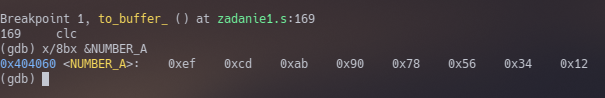
\includegraphics[width=17cm]{Materialy/Lab2/LE}
		\caption{Zapis liczby w pamięci w konwencji Little Endian}
		\label{LE}
	\end{figure}
\end{center}
\subsubsection{Dodawanie liczb z użyciem flagi przeniesienia}
W celu dodania przygotowanych liczb z użyciem rejestrów 64b i flagi CF, należało najpierw wyczyścić flagę przeniesienia (operacja \textbf{clc}), a następnie zapisać rejestr flag na stosie (\textbf{pushf}). Następnie wystarczyło w pętli pobierać po 8 bajtów z buforów zawierających przygotowane liczby i dodawać je za pomocą operacji \textbf{adcq}. Wynik zapisywany był w przygotowanym buforze. Kod przedstawiono na listingu:
\begin{minted}{gas}
	clc # Czyszczenie flagi przeniesienia
	pushf # Zapis rejestru flag na stosie
	# Licznik co 8 bajtów
	xor %r13, %r13
	add_loop:
	movq NUMBER_A(,%r13, 8), %rax # Pobranie 8 bajtów liczby A
	movq NUMBER_B(,%r13, 8), %rbx # Pobranie 8 bajtów liczby B
	popf # Pobranie zawartości rejestru flag ze stosu
	# Operacja dodawania z uwzględnieniem flagi przeniesienia
	adcq %rbx, %rax
	pushf # Zapis rejestru flag na stosie
	movq %rax, SUM(,%r13,8) # Zapis wyniku do bufora
	addq $8, %r13
	cmpq $512, %r13 
	jne add_loop # Warunek końca pętli
	
	# Uwzględnienie przeniesienia po ostatnim dodawaniu
	popf
	movb $0, SUM(,%r13,1)
	jnc convert_sum_to_ascii
	movb $1, SUM(,%r13,1)
\end{minted}
\subsubsection{Zapis wyniku do pliku w postaci ósemkowej}
Zapis wyniku do pliku w postaci ósemkowej zrealizowany został w oparciu o informacje zawarte w pliku PrzykladoweZadania.pdf na stronie kursu. Algorytm działa w oparciu o bazy skojarzone. Grupuje on bajty sumy po 3 (zaczynając od najmłodszych bitów), skleja je w jednym rejestrze, a następnie wyłuskuje kolejne trójki bitów i przetwarza je na kody ASCII.  Dzięki temu za pomocą jednej pętli możliwa jest konwersja liczby na system ósemkowy i zapisanie jej w kodzie ASCII. Kod przedstawiono na listingu:
\begin{minted}{gas}
	convert_sum_to_ascii:
	xor %r14, %r14 # Licznik od początku sumy
	movq $1367, %r15 # Licznik od końca bajtów skonwertowanego wyniku
	merge_3B:
	xor %rax, %rax
	xor %rbx, %rbx
	xor %rcx, %rcx
	movb SUM(,%r14,1), %al # Pierwszy bajt sumy do %rax
	incq %r14 
	movb SUM(,%r14,1), %bl # Kolejny bajt do %rbx
	shl $8, %rbx # Przesunięcie w lewo o 8 bitów zawartości %rbx
	incq %r14
	movb SUM(,%r14,1), %cl # Trzeci bajt do %rcx
	shl $16, %rcx # Przesunięcie w lewo o 16 bitów zawartości %rcx
	orq %rcx, %rbx # Sklejenie %rcx z %rbx
	orq %rbx, %rax # Sklejenie %rbx (%cx + %rbx) z %rax
	
	xor %r8, %r8 # Licznik pętli do 8
	convert_24b_and_save:
	xor %rbx, %rbx
	movb %al, %bl # Kopia bajtu do %bl
	# Wyłuskanie 3 najmłodszych bitów - wartości cyfry w systemie ósemkowym
	andb $0x7, %bl
	shr $3, %rax # Przesunięcie zawartości %rax o 3 bity w prawo
	addb $'0', %bl # Konwersja na kod ASCII
	movb %bl, RESULT(,%r15,1) # Zapisanie do bufora wyjściowego
	decq %r15
	incq %r8
	cmpq $8, %r8
	jl convert_24b_and_save
	incq %r14
	cmpq $513, %r14
	jne merge_3B
	
	# Dopisanie znaku końca linii na końcu wyniku
	movq $1368, %rax
	movb $'\n', RESULT(,%rax,1)
\end{minted}
\subsubsection{Zapis wyniku do pliku}
Zapis do pliku w języku GNU Assembler jest podobny do odczytu. Operacje różnią się między sobą wykorzystanymi funkcjami systemowymi oraz kodami uprawnień. Dla zapisu należało skorzystać z wartości 0101 w \textbf{\%rsi} (zapis oraz stworzenie pliku, jeśli nie istnieje) oraz 0644 w rejestrze \textbf{\%rdx} (bieżący użytkownik otrzymał uprawnienia do zapisu).
\subsection{Wnioski}
Przetwarzanie plików w języku assembler nie jest operacją łatwą. Wymaga od programisty wiedzy dotyczącej uprawnień do operacji na plikach. Zadania zrealizowane w trakcie laboratorium działały poprawnie dla kilku przykładów testowych. Przygotowane programy pozwoliły utrwalić wiedzę zdobytą wcześniej oraz zdobyć nowe informacje z zakresu operacji na plikach.
\newpage
\section{(3) Funkcje}
\subsection{Treść ćwiczenia}
\textbf{Zakres i program ćwiczenia:}
Przygotowanie funkcji realizujących następujące zadania:
\begin{enumerate}
	\item sprawdzenie, czy w podanym łańcuchu znaków znajduje się ciąg "aaa" i zwrócenie indeksu początku tego ciągu lub -1. 
	\item funkcja rekurencyjna (argumenty i wynik przekazywane przez rejestry):
	\begin{equation}
		f(x)=\begin{cases}
			5, & \text{if x = 0}.\\
			2, & \text{if x = 1}.\\
			3*f(x-1)-2*f(x-2), & \text{w pozostałych przypadkach}.
		\end{cases}
	\end{equation}
	\item funkcja rekurencyjna z punktu 2. (argumenty i wynik przekazywane przez stos).
\end{enumerate}
\textbf{Zrealizowane zadania:}
Udało się zrealizować wszystkie zadania przewidziane do realizacji w ramach laboratorium.
\subsection{Przebieg ćwiczenia}
\subsubsection{Struktura funkcji}
Funkcje w języku GNU Assembler mają określoną budowę, która przedstawiona została na listingu:
\begin{minted}{gas}
	.type first_function, @function
	first_function:
	
	... # Instukcje realizowane przez funkcję
	
	ret
\end{minted}
Pierwsze dwie linie przedstawionego listingu to deklaracja funkcji. Funkcja zadeklarowana w ten sposób może być wywołana z dowolnego miejsca pisanego programu za pomocą mnemoniku \textbf{call + nazwa funkcji}.\\
Drugim ważnym elementem jest instrukcja \textbf{ret}, która musi być umieszczona na końcu każdej funkcji. umożliwia ona powrót licznika programu do miejsca tuż po instrukcji \textbf{call}.\\
Argumenty funkcji mogą być przekazywane na kilka sposobów:
\begin{itemize}
	\item przez rejestry.
	\item przez zmienne globalne.
	\item przez stos.
\end{itemize}
W zrealizowanych ćwiczeniach zaprezentowane zostały dwa z wymienionych sposobów - przekazywanie przez rejestry oraz przez stos.
\subsubsection{Funkcja sprawdzająca, czy w podanym łańcuchu znaków znajduje się ciąg "aaa"}
W celu przygotowania programu, będącego rozwiązaniem tego zadania nie trzeba było deklarować żadnych nowych stałych w sekcji \textbf{.data}. W sekcji \textbf{.bss} zadeklarowano jeden bufor do przechowania tekstu wejściowego. Łańcuch znaków wczytano za pomocą wywołania systemowego. Przygotowana funkcja przyjmuje dwa argumenty: długość ciągu znaków w rejestrze \textbf{\%r8} oraz adres ciągu znaków w rejestrze \textbf{\%rax}. Jej działanie polega na porównywaniu kolejnych znaków wczytanego łańcucha z literą 'a'. Po wykryciu tej litery trzy razy z rzędu program zwraca indeks pierwszej litery ciągu "aaa". W przeciwnym wypadku zwraca -1. Kod funkcji przedstawiono na listingu:
\begin{minted}{gas}
	.type check, @function # Deklaracja funkcji
	check:
	movq $-1, %r10 # Indeks pierwszego znaku ciągu "aaa"
	subq $1, %r8 # Liczba wczytanych do bufora znaków - 1
	
	first:
	incq %r10
	# Jeżeli indeks pierwszego znaku >= liczbie wczytanych znaków-1
	cmpq %r8, %r10
	# Brak ciągu "aaa"
	jge check_failed
	movb (%rax, %r10, 1), %cl # Wczytanie pierwszego znaku do rejestru %cl
	cmpb $'a', %cl
	je second # Jeżeli wczytany znak to 'a' -> sprawdzaj dalej
	jmp first # Wprzeciwnym razie zacznij od nowa
	
	
	
	# Sprawdzenie drugiego wystąpienia z rzędu litery 'a'
	second:
	incq %r10
	cmpq %r8, %r10
	jge check_failed
	movb (%rax, %r10, 1), %cl 
	cmpb $'a', %cl
	je third
	jmp first
	
	... # Sprawdzenie trzeciego wystąpienia z rzędu litery 'a'
	
	# Nie znaleziono ciągu "aaa" -> funkcja zwraca -1
	check_failed:
	movq $-1, %rbx # Indeks w %rbx
	jmp end
	
	# Znaleziono ciąg "aaa" -> funkcja zwraca indeks pierwszej litery 'a'
	found:
	sub $2, %r10
	movq %r10, %rbx # Indeks w %rbx
	
	end:
	ret # Powrót do miejsca wywołania funkcji
\end{minted}
Wywołanie funkcji odbywa się za pomocą polecenia \textbf{call check}. Znajduje się ono w kodzie programu tuż po przeniesieniu argumentów wywołania funkcji do odpowiednich rejestrów. Wynik zwracany przez funkcję drukowany jest na ekran za pomocą \textbf{printf}.
\begin{minted}{gas}
	xor %rax, %rax # Liczna argumentów zmiennoprzecinkowych
	movq $OUTPUT, %rdi # Adres ciągu wyjściowego
	# Parametr ciągu wyjściowego - indeks pierwszej litery 'a'
	movq %rbx, %rsi 
	call printf
\end{minted}
\subsection{Funkcja rekurencyjna - argumenty i wynik przekazywane przez rejestry}
Funkcja rekurencyjna jest szczególnym rodzajem funkcji - wywołuje ona samą siebie, co czyni ją wyjątkową. Obliczenie jej wartości opiera się na znajomości dwóch pierwszych wartości funkcji. Zadeklarowane są one w kodzie programu jako stałe. Przygotowana funkcja przyjmuje tylko jeden parametr - numer wyrazu ciągu, którego wartość chcemy poznać. Wartość ta trafia do rejestru \textbf{\%r12}. Funkcja sprawdza najpierw, czy użytkownik nie żąda zwrócenia wartości wyrazu 0 lub 1 - jeżeli oczekuje takiej informacji to otrzymuje ją natychmiast z pamięci programu i funkcja zostaje zakończona. W przeciwnym przypadku wartość funkcji obliczana jest poprzez rekurencyjne jej wywoływanie. Wynik ostatecznie trafia do rejestru \textbf{\%rbx} i zostaje wypisany na ekran za pomocą \textbf{printf}. Kod funkcji przedstawiono na listingu:
\begin{minted}{gas}
	.type calculate, @function
	calculate:
	# Jeżeli N = 0 lub N = 1 -> skok do sekcji zwracających stałą
	cmpq $1, %r12
	je returnN1
	jl returnN0
	
	# Zerowanie wyniku
	xor %rcx, %rcx
	decq %r12 # Zmniejszenie wartości N
	pushq %rcx # Umieszczenie wyniku na stosie
	call calculate # Wywołanie rekurencyjne
	popq %rcx # Pobranie wyniku ze stosu
	incq %r12 $ Zwiększenie wartości N
	
	# Przeniesienie wartości zwróconej przez f. rekurencyjną do %rax
	movq %rbx, %rax 
	xor %rdx, %rdx
	mulq %r8 # Mnożenie przez 3
	addq %rax, %rcx # Dodanie do wyniku głównego
	
	subq $2, %r12
	pushq %rcx
	call calculate
	popq %rcx
	addq $2, %r12
	
	movq %rbx, %rax
	xor %rdx, %rdx
	mulq %r9 # Mnożenie przez -2
	addq %rax, %rcx # Dodanie do wyniku głównego
	movq %rcx, %rbx # Wynik funkcji w %rbx
	jmp end
	
	returnN1:
	movq %r11, %rbx # Zwrócenie wartości dla 1. wyrazu ciągu
	jmp end
	
	returnN0:
	movq %r10, %rbx # Zwrócenie wartości dla 0. wyrazu ciągu
	
	end:
	ret
\end{minted}
\subsubsection{Funkcja rekurencyjna - argumenty i wynik przekazywane przez stos}
Wykorzystanie stosu programowego w funkcjach wymaga umieszczenia na stosie wartości rejestru bazowego \textbf{\%rbp} oraz pobrania zawartości rejestru zawierającego wskaźnik na ostatni element umieszczony na stosie (\textbf{\%rsp}) do rejestru bazowego. Przed zakończeniem działania funkcji konieczne odwrócenie tego działania. Argumenty funkcji przekazywane są przez stos za pomocą polecenia \textbf{push}, zaś wynik pobierany jest za pomocą polecenia \textbf{pop}. Przygotowana funkcja wygląda podobnie do poprzedniej, jednak zmienia się mocno sposób wywoływania rekurencyjnego funkcji - należy wysyłać i pobierać ze stosu znacznie więcej danych, co pokazano na listingu:
\begin{minted}{gas}
	.type calculate, @function
	calculate:
	pushq %rbp # Rejestr bazowy na stos
	movq %rsp, %rbp # Stack pointer do rejestru %rbp
	movq 16(%rbp), %r8 # Wartość N do rejestru %r8
	
	... # Porównanie do stałych
	
	xor %rcx, %rcx
	decq %r8
	pushq %rcx # Wynik na stos
	pushq %r8 # Wartość N na stos
	call calculate
	popq %rbx # Pobranie wyniku poprzedniego wywołania
	popq %rcx # Pobranie wyniku głównego
	incq %r8

	... # Mnożenie przez 3
	
	subq $2, %r8
	pushq %rcx
	pushq %r8
	call calculate
	popq %rbx
	popq %rcx
	addq $2, %r8
	
	,.. # Mnożenie przez -2
	
	... # Zwrócenie stałych wartości
	
	end:
	movq %rbx, 16(%rbp) # Wynik na stosie
	# Przywracanie porządku
	movq %rbp, %rsp
	popq %rbp
	ret
\end{minted}
\subsection{Wnioski}
Funkcje pozwalają na znaczne zmniejszenie ilości kodu powtarzającego się często w programie. Umożliwiają również dodanie nowych funkcjonalności w innych programach bez konieczności tworzenia nowego kodu. Obsługa stosu programowego nie należy do zadań łatwych - jego skuteczne wykorzystanie wymaga od programisty świetnego zrozumienia zasady jego działania i umiejętności określenia, co w danej chwili znajduje się na stosie. Zrealizowane zadania pozwoliły na przyswojenie wiedzy z zakresu pisania funkcji i obsługi stosu, co na pewno pozwoli na uproszczenie programów pisanych w przyszłości. Przygotowane aplikacje wykonały się poprawnie i nie zwracały żadnych błędów.
\newpage
\section{(4) Łączenie różnych języków programowania w jednym projekcie}
\subsection{Treść ćwiczenia}
\textbf{Zakres i program ćwiczenia:}
Przygotowanie programów realizujących następujące zadania:
\begin{enumerate}
	\item Program w języku assemblera:
	\begin{itemize}
		\item wczytanie liczby zmiennoprzecinkowej x i całkowitoliczbowej y za pomocą funkcji scanf.
		\item wywołanie funkcji napisanej w języku C: $f(x,y) = x^2+y^3$.
		\item wypisanie wyniku na ekran (liczba zmiennoprzecinkowa i jej część całkowita(int)) za pomocą funkcji \textbf{printf}.
	\end{itemize}
	\item Program w języku C, wywołujący funkcję napisaną w języku assemblera - szyfr Cezara dla cyfr i zadanego klucza.
	\item Wstawka assemblerowa, realizująca zadanie z punktu 2.
\end{enumerate}
\textbf{Zrealizowane zadania:}
W trakcie laboratorium udało się zrealizować zadania numer 1 i 2. Na zadanie 3 zabrakło czasu, jednak udało się je zrealizować w warunkach domowych. 
\subsection{Przebieg ćwiczenia}
\subsubsection{Program w języku assemblera wywołujący funkcję napisaną w języku C}
Realizację tego programu rozpoczęto od próby wczytania liczby zmiennoprzecinkowej oraz całkowitoliczbowej za pomocą funkcji \textbf{scanf}. Zadanie to okazało się bardzo proste. Wystarczyło tylko w sekcji \textbf{.data} zapisać odpowiedni łańcuch formatujący, a następnie wywołać funkcję \textbf{scanf} z właściwie przekazanymi parametrami. Prawidłowe rozwiązanie pokazano na listingu:
\begin{minted}{gas}
	.data
	FORMAT: .asciz "%d %f" # Łańcuch formatujący
	
	.bss
	# Bufory dla liczby całkowitoliczbowej i zmiennoprzecinkowej
	.comm INTEGER_INPUT, 4
	.comm FLOAT_INPUT, 4
	
	.text
	.globl main
	
	main:
	
	# Liczba parametrów zmiennoprzecinkowych przekazywanych do funkcji
	xor %rax, %rax 
	movq $FORMAT, %rdi # Łańcuch foramtujcy do %rdi
	movq $INTEGER_INPUT, %rsi # Adres bufora liczby całkowitoliczbowej
	movq $FLOAT_INPUT, %rdx # Adres bufora liczby zmiennoprzecinkowej
	call scanf # Wywołanie funkcji
\end{minted}
Kolejnym krokiem było przygotowanie funkcji w języku C, która zostanie później wywołana z poziomu assemblera. Jej treść przedstawiono na listingu:
\begin{minted}{c}
	double calculate(int a, float b){
		return a*a+b*b*b;
	}
\end{minted}
Funkcja jest niezwykle prosta - zwraca sumę kwadratu liczby całkowitoliczbowej i sześcianu liczby zmiennoprzecinkowej. Wynikiem tej funkcji jest liczba typu double.\\
Wywołanie funkcji napisanej w języku C z poziomu assemblera  wymaga podania ilości argumentów zmiennoprzecinkowych oraz umieszczenia wszystkich parametrów wywoływanej funkcji w odpowiednich rejestrach. Prawidłowe wywołanie pokazano na listingu:
\begin{minted}{gas}
	movq $1, %rax # Liczba argumentów zmiennoprzecinkowych
	xor %rdx, %rdx 
	xor %rcx, %rcx
	# Argument całkowitoliczbowy do rejestru %edi
	movl INTEGER_INPUT(,%rcx,4), %edi
	# Argument zmiennoprzecinkowy do rejestru %xmm0
	movss FLOAT_INPUT, %xmm0
	call calculate
\end{minted}
Wynik wywołanej funkcji znajduje się w rejestrze \textbf{\%xmm0}. Aby wydrukować go na ekran za pomocą funkcji \textbf{printf}, należy zastosować obejście w celu zabezpieczenie ostatniej komórki na stosie przed zmianą. Od wskaźnika stosu należy odjąć wartość równą 8 * ilość parametrów zmiennoprzecinkowych. W przypadku drukowania wartości całkowitoliczbowych stosowanie obejścia nie jest wymagane, co pokazano na listingu:
\begin{minted}{gas}
	# Drukowanie liczby zmiennoprzecinkowej
	movq $1, %rax # Liczba parametrów zmiennoprzecinkowych
	movq $FORMAT_O, %rdi # Łańcuch formatujący
	subq $8, %rsp # Obejście
	call printf
	addq $8, %rsp # Obejście
	
	# Drukowanie liczby całkowitoliczbowej
	movq $0, %rax # Liczba parametrów zmiennoprzecinkowych
	movq $FORMAT_1, %rdi # Łańcuch formatujący
	xor %rcx, %rcx
	xor %rsi, %rsi
	movl INTEGER_INPUT(,%rcx,4), %esi # Argument funkcji do %esi
	call printf
\end{minted}
\newpage
\subsubsection{Program w języku C, wywołujący funkcję napisaną w języku assemblera}
Przygotowanie programu, realizującego szyfr Cezara dla cyfr i zadanego klucza rozpoczęto od stworzenia pliku źródłowego w języku C. Zawiera on deklarację zewnętrznej funkcji, definicje stałych wykorzystywanych w programie oraz sekcję \textbf{main}, w której wywoływana jest funkcja napisana w języku assemblera. Wynik jest zaś drukowany na ekran za pomocą funkcji \textbf{printf}.\\
Znacznie ciekawszy jest plik źródłowy, napisany w języku GNU Assembler. Zawiera on definicję funkcji, realizującej szyfr Cezara, którą wywołać można we wcześniej przygotowanym pliku napisanym w języku C. Aby coś takiego było możliwe, konieczne było zdefiniowanie punktu wejścia programu na \textbf{.globl caesar}, gdzie caesar jest nazwą przygotowanej funkcji. Przedstawiono to na listingu:
\begin{minted}{gas}
	.data
	
	.text
	.type caesar, @function
	.globl caesar
	caesar:
	pushq %rbp
	movq %rsp, %rbp
	
	... # Kod funkcji
	
	movq %rbp, %rsp
	popq %rbp
	ret
\end{minted}
Algorytm funkcji bazuje wyłącznie na wiedzy z poprzednich laboratoriów, dlatego nie został opublikowany w sprawozdaniu. Jest to prosta pętla, w której po kolei pobierane są bajty ciągu wejściowego. Następnie są sprawdzane, czy są liczbami. Jeśli tak to dodawana jest do nich wartość zadanego klucza. Wynik jest dzielony przez 10, w celu uniknięcia przekroczenia zakresu 0-9, a następnie zapisywany z powrotem w ciągu wejściowym. Argumenty funkcji przekazywane są przez rejestry \textbf{\%rdi} (adres początku ciągu testowego), \textbf{\%rsi} (długość ciągu wejściowego) oraz \textbf{\%rdx} (klucz szyfrujący).
\subsubsection{Program w języku C z wstawką assemblerową}
Przygotowany program realizuje dokładnie to samo zadanie, co w punkcie poprzednim - jest to szyfr Cezara z zadanym kluczem. Jednakże tym razem zamiast łączyć dwa pliki źródłowe, wykorzystano fragmenty kodu w języku assemblera bezpośrednio wewnątrz pliku z kodem źródłowym, napisanym w języku C. Aby było to możliwe, w funkcji \textbf{main} umieszczono sekcję \textbf{asm()}, w której znajduje się kod napisany w języku GNU Assembler. Struktura takiej wstawki jest następująca:
\begin{enumerate}
	\item Linijki kodu w znakach "" i zakończone znakiem nowej linii \textbf{\textbackslash n}. Rejestry w tym kodzie oznaczać należy za pomocą podwójnego znaku \textbf{\%}, np. \textbf{\%\%rax}.
	\item : lista zmiennych wyjściowych.
	\item : lista zmiennych wejściowych. Zmienne te muszą mieć zdefiniowany sposób przekazywania. Na przykład, jeżeli chcemy przechować argument wejściowy w rejestrze \textbf{\%edi} to zmienną należy zdefiniować w następujący sposób: \textbf{"D"(test\_string)}, gdzie test\_string jest nazwą przekazywanej zmiennej. W celu poznania innych sposobów przekazywania odsyłam do innych źródeł. 
	\item : lista rejestrów wykorzystanych we wstawce. 
\end{enumerate}
Aby odwołać się do parametru wejściowego wewnątrz wstawki assemblerowej, należy skorzystać z notacji \textbf{\%N}, gdzie N jest numerem argumentu wejściowego, licząc od 0, np. \textbf{\%0, \%1}, itd.\\
Wewnątrz wstawki można również korzystać ze stałych, zdefiniowanych w kodzie źródłowym, napisanym w języku C. Wystarczy odwołać się do stałej poprzez nazwę, np. aby porównać stałą \textbf{test\_len} z zwartością rejestru \textbf{\%ecx} wystarczy napisać następujący fragment kodu:
\begin{minted}{gas}
	"cmp test_len, %%ecx\n"
\end{minted}
Sam algorytm nie zmienia się praktycznie względem funkcji wcześniej napisanej w pliku źródłowym języka GNU Assembler. Zmianie uległa jedynie składnia.
\subsection{Wnioski}
Możliwość łączenia kodu C i Assemblera jest bardzo cenną funkcjonalnością, szczególnie dla programistów C. Użycie języka assemblera może w wielu przypadkach znacznie przyspieszyć działanie tworzonej aplikacji. Wszystkie przygotowane programy działały poprawnie dla danych testowych. Ich przygotowanie pozwoliło utrwalić wcześniej zdobytą wiedzę z zakresu pisania funkcji oraz rozszerzyć ją o kilka nowości, takich jak eksport funkcji napisanej w języku assemblera do programu napisanego w języku C. Jedyny problem, jaki pojawił się w procesie tworzenia programów dotyczył warunku zakończenia pętli we wstawce assemblerowej. Przez niedopatrzenie programisty dochodziło do próby porównania liczby typu int (32b) z zawartością rejestru 64b, co powodowało nieskończoną pracę pętli, a w efekcie błąd programu. Zmiana rejestru 64b na 32b (w tym przypadku \textbf{\%ecx}) umożliwiła poprawne wykonanie programu. Warto wspomnieć, że debugowanie programu złożonego z dwóch plików źródłowych okazało się bardzo trudnym zadaniem, brak dostępu do kodu assemblerowego praktycznie uniemożliwiał zlokalizowanie błędu.
\newpage  
\section{(5) Jednostka zmiennoprzecinkowa (FPU)}
\subsection{Treść ćwiczenia}
\textbf{Zakres i program ćwiczenia:}
Przygotowanie programów realizujących następujące zadania:
\begin{enumerate}
	\item Funkcja w języku assemblera, obliczająca wartość funkcji arctg(x), korzystając z rozwinięcia szeregu Taylora.
	\item Funkcja w ASM sprawdzająca wskazaną flagę (dla określonego wyjątku) w Status Word.
	\item Funkcja w ASM modyfikująca ustawienia maskowania wyjątków w Control Word (dla wskazanego wyjątku).
	\item Wykazanie różnicy dla maskowania i nie maskowania wyjątków.
\end{enumerate}
\textbf{Zrealizowane zadania:}
Udało się zrealizować wszystkie zadania przewidziane do realizacji w ramach laboratorium.
\subsection{Przebieg ćwiczenia}
\subsubsection{Obliczenie wartości funkcji arctg(x), korzystając z rozwinięcia szeregu Taylora}
W celu przygotowania funkcji obliczającej wartość arctg(x), korzystając z rozwinięcia szeregu Taylora należało najpierw wyszukać odpowiedni wzór matematyczny, który pozwoli na realizację tego zadania. Przedstawiono go na \textit{rysunku 3}.
\begin{center}
	\begin{figure}[h]
		\centering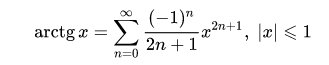
\includegraphics[width=10cm]{Materialy/Lab5/taylor}
		\caption{Rozwinięcie szeregu Taylora dla funkcji arctg(x)}
		\label{taylor}
	\end{figure}
\end{center}
X we wzorze oznacza kąt w stopniach, zaś n - liczbę powtórzeń operacji sumowania.\\\\
Funkcję w języku assemblera przygotowano z wykorzystaniem rozkazów koprocesora arytmetycznego(FPU). Jednostka zmiennoprzecinkowa charakteryzuje się tym, że posiada własny zestaw rejestrów, działających na zasadzie magazynku w rewolwerze. Po zrozumieniu zasady działania tych rejestrów i zapoznaniu się z listą rozkazów koprocesora przygotowana została następująca funkcja, realizująca wzór z \textit{rysunku 3}:
\begin{minted}{gas}
	.data
	two : .double 2.0
	
	.text
	.type arctgx, @function
	.global arctgx
	arctgx:
	pushq %rbp
	movq %rsp, %rbp
	
	finit # Inicjacja jednostki zmiennoprzecinkowej
	sub $8, %rsp 
	# Załadowanie kąta do rejestru ST0
	movsd %xmm0, (%rsp)
	fldl (%rsp)
	fst %st(1) # Kopiowanie ST0 do ST1
	fst %st(2)
	fst %st(3)
	fld1 # Załadowanie liczby 1 do ST0
	fxch %st(1) # Zamiana wartości ST0 z ST1
	
	# Zawartość rejestrów na początku funkcji:
	# ST4 - X
	# ST3 - Wynik - X na początku
	# ST2 - Wyraz ciągu - X na początku
	# ST1 - Mianownik ułamka - 1.0 na starcie
	# ST0 - Licznik ułamka - X na początku
	
	movq $0, %r8 # Aktualna wartość licznika pętli
	
	loop:
	cmpq %rdi, %r8
	# Warunek końca pętli licznik = parametrowi n
	je end
	incq %r8
	
	
	# Obliczenie wartości licznika
	fchs # Zmiana znaku licznika
	# Dwukrotne mnożenie licznika przez X
	fmul %st(4), %st
	fmul %st(4), %st
	
	# Obliczenie wartości mianownika
	fxch %st(1) # Zamiana ST0 z ST1
	faddl two # Dodanie liczby 2.0 do ST0
	fxch %st(1) # Ponowna zamiana ST0 z ST1
	
	# Obliczenie wartości wyrazu ciągu
	fst %st(2) # Kopiowanie ST0 do ST2
	fdiv %st(1), %st # Dzielenie ST0/ST1
	fadd %st, %st(3) # Dodanie wyrazu ciągu do wyniku ogólnego
	fxch %st(2) # Zamiana ST0 z ST2 - porządkowanie
	
	jmp loop
	
	end:
	fxch %st(3) # Wynik do ST0
	# Wysłanie wyniku do rejestru %xmm0 przez stos
	fstpl (%rsp) 
	movsd (%rsp), %xmm0
	
	movq %rbp, %rsp
	popq %rbp
	ret
\end{minted}
Przygotowana funkcja działała poprawnie i zwracała dobre wyniki dla różnych przypadków testowych. Kod źródłowy w języku C nie wnosi niczego nowego - zawiera wywołanie funkcji napisanej w języku assemblera.
\subsubsection{Funkcja w ASM sprawdzająca Status Word}
FPU zawiera trzy 16-bitowe rejestry specjalne - Status Word, Control Word oraz Tag Word. Status Word zawiera flagi, które pozwalają opisać aktualny stan koprocesora FPU. Poszczególne jego bity odpowiadają za różnego rodzaju wyjątki, takie jak: nieprawidłowa operacja, zdenormalizowany operand, dzielenie przez zero, czy przeciążenie. W celu pobrania aktualnej wartości Status Word, należało przygotować bardzo prostą funkcję:
\begin{minted}{gas}
	.type getStatus, @function
	getStatus:
	pushq %rbp
	movq %rsp, %rbp
	
	xor %rax, %rax
	fstsw status # Pobranie Status Word do bufora status
	mov status, %ax # Zapisanie Status Word w rejestrze %ax
	
	movq %rbp, %rsp
	popq %rbp
	ret
\end{minted}
Wywołanie takiej funkcji z poziomu programu w języku C pozwala podejrzeć wartość liczbową rejestru Status Word, a co za tym idzie - umożliwia dostęp do aktualnych wartości flag koprocesora FPU. Wywołanie funkcji z poziomu języka C domyślnie zwraca wartość 0, jednak przy próbie dzielenia przez 0 wartość ta ustawia się na 14340.
\subsubsection{Funkcja w ASM modyfikująca ustawienia maskowania wyjątków w Control Word}
Control Word jest kolejnym rejestrem specjalnym jednostki zmiennoprzecinkowej. Pozwala na zarządzanie maskowaniem wyjątków, kontrolą precyzji obliczeń oraz trybu zaokrąglania wyników. Podgląd jego wartości odbywa się podobnie do Status Word, z tą różnicą, że zamiast operacji \textbf{fstsw} należy użyć mnemoniku \textbf{fstcw}.\\
W celu modyfikacji ustawień maskowania wyjątków w Control Word konieczne było przygotowanie bardzo obszernego programu w języku C, pełniącego funkcję interfejsu użytkownika. Kod ten opiera się głownie o szereg instrukcji switch/case oraz wywołań funkcji \textbf{printf}, dlatego też nie zostanie zaprezentowany w sprawozdaniu. Wywołanie funkcji zarządzającej maskowanie wyjątków zawiera dwa argumenty: numer porządkowy wyjątku (od 0 do 5 - analogicznie do numeru bitu wyjątku w CW)) oraz wartość maski wyjątku (0 dla nieustawionej oraz 1 dla ustawionej). Proces ustawiania maski wyjątku dzielenia przez 0 zaprezentowano na listingu:
\begin{minted}{c}
	case 3:
		printf("Zero divide exception mask\n");
		printf("1 - Unset\n");
		printf("2 - Set\n");
		scanf("%d", &set);
		if(set==1){
			setControl(2,0);
		}
		else
		{
			setControl(2,1);
		}
		printf("\n Current Control Word: %hd \n\n\n", getControl());
		break;
\end{minted}
Funkcja w języku assemblera, modyfikująca Control Word jest bardzo prosta, ale przy tym dość obszerna, w związku z czym zaprezentowany zostanie tylko jej wycinek dla maski dzielenia przez zero. Na początku funkcja pobiera do rejestru \textbf{\%ax} aktualną wartość Control Word. Następnie sprawdza pierwszy podany argument i lokalizuje, która maska ma zostać zmodyfikowana. Na koniec na podstawie drugiego argumentu ustawia maskę na 0 lub 1 oraz zapisuje nową wartość rejestru Control Word. Przykład modyfikacji pokazano na listingu:
\begin{minted}{gas}
	.type setControl, @function
	setControl:
	pushq %rbp
	movq %rsp, %rbp
	
	# Pobranie wartości Control Word
	fstcw control
	mov control, %ax
	
	# Sprawdzenie pierwszego argumentu i skok warunkowy
	cmpq $2, %rdi
	je ZERO_DIVIDE
	
	... # Porównanie pierwszego argumentu z id pozostąłych wyjątków
	
	# W przypadku podania wartości > 5 funkcja nic nie zrobi
	jmp END
	

	# Zarządzanie maską dzielenia przez zero
	ZERO_DIVIDE:
	cmpq $0, %rsi
	jg SET_ZERO
	
	# Ustawienie maski na 0
	and $0xFFFB, %ax
	jmp END
	
	SET_ZERO:
	# Ustawienie maski na 1
	or $0x4, %ax
	jmp END
	
	
	... # Ustawiania masek innych wyjątków
	
	END:
	mov %ax, control
	# Zapis nowego Control Word
	fldcw control
	movq %rbp, %rsp
	popq %rbp
	ret
\end{minted}
Tak przygotowana funkcja umożliwia sprawne zarządzanie rejestrem Control Word, co pokazano na \textit{rysunku 5}:
\begin{center}
	\begin{figure}[h]
		\centering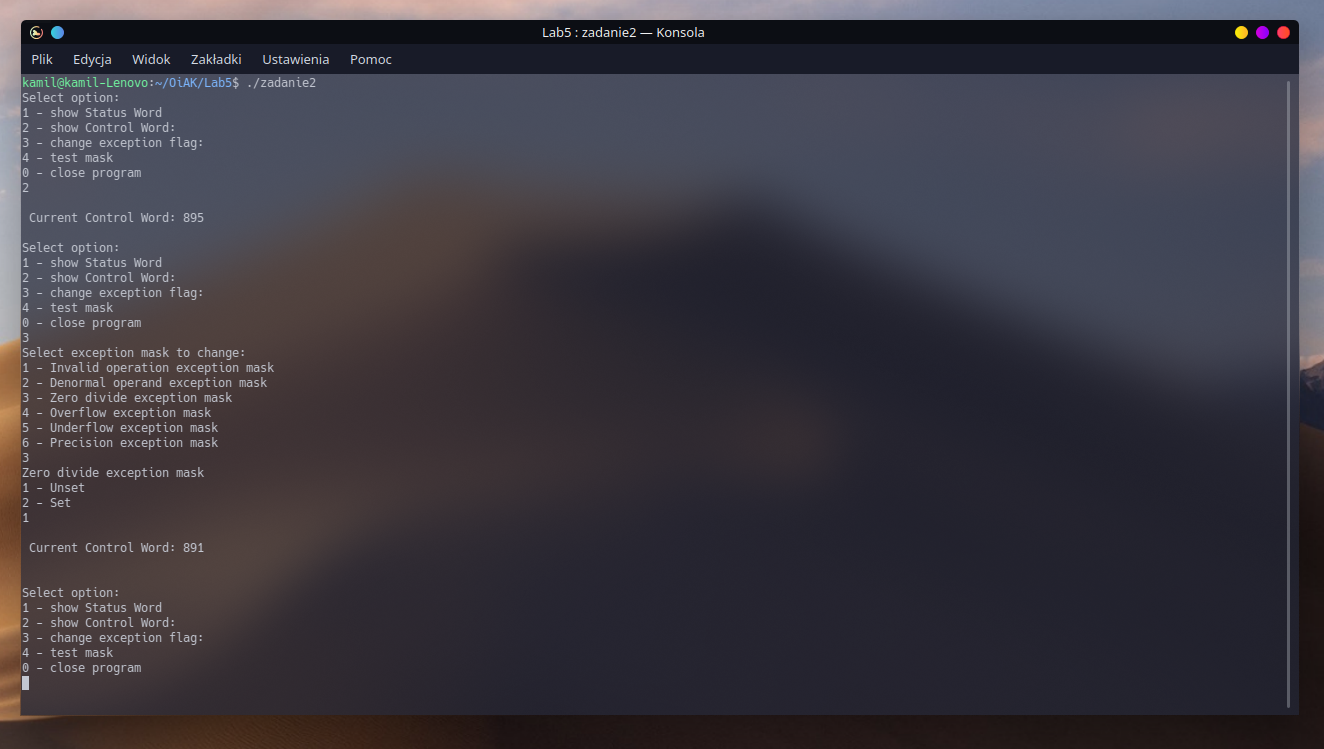
\includegraphics[width=17cm]{Materialy/Lab5/maska}
		\caption{Kontrola maskowania wyjątków w Control Word}
		\label{maska}
	\end{figure}
\end{center}
\newpage
\subsubsection{Wykazanie różnicy dla maskowania i nie maskowania wyjątków}
W celu pokazania różnicy pomiędzy maskowaniem i nie maskowanie wyjątków jednostki zmiennoprzecinkowej przygotowano prostą operację testową, pokazaną na listingu:
\begin{minted}{gas}
	.type checkError, @function
	checkError:
	pushq %rbp
	movq %rsp, %rbp
	
	finit
	# Załadowanie 1.11 do rejstru FPU
	flds float
	# Próba dzielenia przez 0.00
	fdiv zero
	
	movq %rbp, %rsp
	popq %rbp
	ret
\end{minted}
Wywołanie tej funkcji dla ustawionej i nie ustawionej maski dzielenia przez zero daje różne wyniki, co zaprezentowano na \textit{rysunku 6}.
\begin{center}
	\begin{figure}[h]
		\centering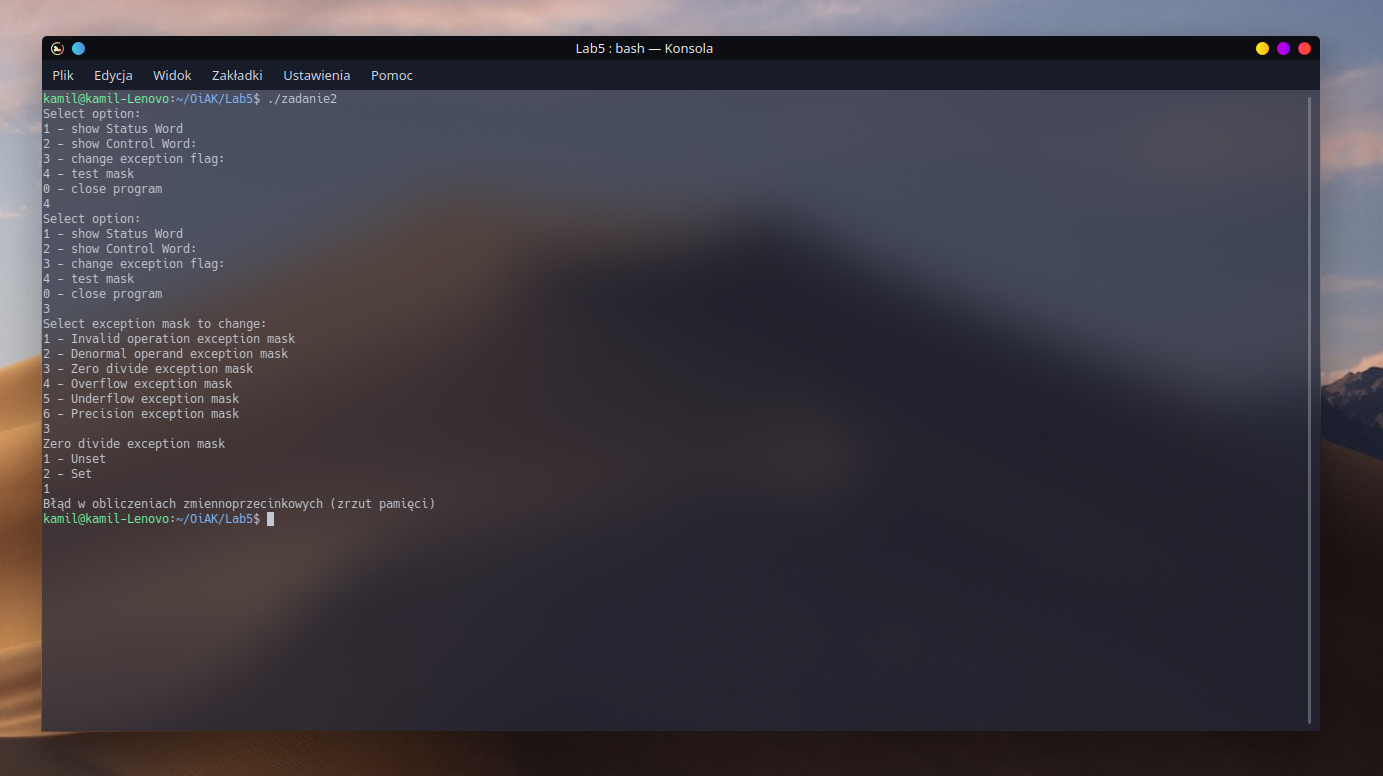
\includegraphics[width=17cm]{Materialy/Lab5/check}
		\caption{Różnica pomiędzy maskowaniem i nie maskowaniem wyjątku dzielenia przez zero}
		\label{check}
	\end{figure}
\end{center}
Po uruchomieniu programu wartość maski dzielenia przez 0 ustawiona jest na 1. Wywołanie funkcji testowej nie zwraca żadnego błędu. W momencie zmiany maski dzielenia przez 0 na 0 automatycznie program zwraca błąd w obliczeniach zmiennoprzecinkowych.
\subsection{Wnioski}
Jednostka zmiennoprzecinkowa to bardzo ciekawe narzędzie, umożliwiające wykonywanie skomplikowanych obliczeń na liczbach zmiennoprzecinkowych. W celu realizacji zadania niezbędne było zapoznanie się z opisem jednostki FPU oraz jej rejestrów specjalnych. Wiedza zdobyta podczas pozostałych laboratoriów uzupełniona o nowe informacja umożliwiła przygotowanie ciekawej aplikacji, obliczającej wartość funkcji arctg(x) z rozwinięcia szeregu Taylora. Wszystkie przygotowane programy działały zgodnie z założeniami i zwracały poprawne wyniki.
\end{document}